\chapter{Progetto di stage}
\label{cap:stage}

\section{Il progetto}

Wintech all'evento di StageIT portava tre proposte riguardanti dei progetti legati alle unità di \emph{business} e sviluppo. Durante la breve discussione avuta in fiera, tra i vari dipendenti era presente anche Mirco, del \emph{team} di \emph{network}, con cui è emersa la possibilità di avviare un progetto legato a questo ambito. Dopo un primo scambio di \emph{mail} per capire meglio le esigenze e le possibilità, è stato fissato un incontro in azienda per discutere meglio del progetto con il responsabile e mio futuro tutor Roberto Pezzile.

Nell'ultimo periodo l'azienda si stava informando e analizzando il mercato alla ricerca di uno strumento di NDR da integrare nella propria rete in modo da aumentare le capacità di rilevazione e risposta agli attacchi informatici. Avendo una grande quantità di clienti in \emph{full-outsourcing} che affidano la gestione della propria infrastruttura a Wintech è necessario avere strumenti di sicurezza sempre aggiornati che sfruttano le ultime tecnologie.

Un sistema di NDR è uno strumento che consente di individuare rapidamente i pericoli nella rete e di attuare una \emph{remediation} automatica. Questo monitora costantemente il traffico tramite sonde posizionate in punti strategici e analizza i dati raccolti per identificare eventuali attività sospette o pericolose. In caso di pericolo, il sistema può attivare una risposta automatica o notificare un amministratore, consentendo di rispondere in modo rapido ed efficace ai potenziali attacchi. Questa tipologia di prodotti offre la possibilità di integrarsi con il resto dell'infrastruttura esistente, principalmente con \emph{firewall} e altri componenti di rete, ma anche con \emph{software} presenti sui vari \emph{host}, sia che questi siano \emph{client} o \emph{server}. Lo scopo del progetto è quello di andare a mettere in produzione uno strumento di questo tipo, già individuato dall'azienda, inizialmente come \emph{Proof of Concept} e successivamente come strumento di sicurezza per i clienti in \emph{full-outsourcing}.

Questo particolare tipo di tecnologia viene proposto da aziende affermate sul mercato della strumentazione di rete, ma la scelta di Wintech è stata quella di puntare su \emph{Sangfor}, un nuovo \emph{player} che cerca di affermarsi con prodotti innovativi e competitivi. Tra i principali punti di forza di questa collaborazione si trovano una maggiore economicità ma specialmente la possibilità di instaurare un dialogo molto più diretto con il fornitore rispetto a grandi corporazioni multinazionali dalla lunga storia. Il periodo scelto per lo stage ha permesso inoltre di sfruttare come banco di prova per il sistema l'infrastruttura di un cliente che gestisce strutture ricettive in un periodo di alta stagione, in cui la rete viene messa a dura prova da un gran numero di utenti con esigenze diverse.

Personalmente, ho avuto modo di avere un contatto diretto con esponenti di Sangfor del \emph{team} italiano della sede di Milano, principalmente remoto e digitale e con un'incontro in sede, e con il \emph{team} di supporto remoto asiatico, che si è reso sempre disponibile per risolvere i problemi riscontrati, anche scontrandosi con fusi orari e lingue diverse.

\section{Vincoli}

\subsection{Vincoli tecnologici}

Gli unici vincoli tecnologici posti da Wintech sono stati quelli di utilizzare strumentazione già scelta da loro, dato che il fornitore del prodotto era già stato definito e i vari strumenti di rete erano già in uso, collaudati e non era possibile andare a sostituirli senza una forte motivazione, vista la complessità dell'operazione, sia dal punto di vista tecnico che economico.

\subsection{Vincoli temporali}

Il progetto di stage è stato pianificato per una durata di 320 ore, suddivise in 8 settimane, con un impegno di 40 ore settimanali. Questo ha permesso di avere un quadro generale del lavoro da svolgere e delle tempistiche da rispettare per arrivare ad avere un prodotto configurato e documentato entro le scadenze.

Nella \autoref{tab:fasi-progetto} troviamo un prospetto orario suddiviso per le varie fasi del progetto individuate e relativo diagramma di Gantt in \autoref{fig:gantt}. Queste verranno descritte nel dettaglio nella \autoref{sec:pianificazione}.

\begin{table}[!htbp]
    \centering
    \begin{tabularx}{\linewidth}{Xccc}
        \toprule
        {\textbf{Fase}} & \textbf{Inizio} & \textbf{Fine} & \textbf{Ore} \\
        \midrule
        Introduzione ed analisi dello strumento e dell'infrastruttura aziendale & 05/06/2023 & 09/06/2023 & 40 \\
        Deploy e configurazione dello strumento, formazione riguardante tutti gli strumenti necessari per la comprensione delle minacce & 12/06/2023 & 23/06/2023 & 80 \\
        Test del prodotto, analizzando rischi ed attacchi reali e/o simulati & 26/06/2023 & 07/07/2023 & 80 \\
        Configurazione e test delle \emph{remediation} & 10/07/2023 & 21/07/2023 & 80 \\
        Stesura della documentazione interna sulle \emph{feature}, l'installazione e l'utilizzo del prodotto & 24/07/2023 & 28/07/2023 & 40 \\
        \bottomrule
    \end{tabularx}
    \caption{Fasi del progetto di stage}
    \label{tab:fasi-progetto}
\end{table}

\begin{figure}[!htbp]
    \centering
    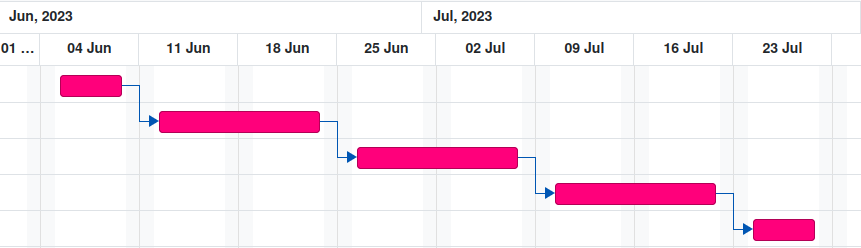
\includegraphics[width=\textwidth]{../images/gantt.png}
    \caption{Diagramma di Gantt delle fasi del progetto di stage}
    \label{fig:gantt}
\end{figure}

\subsection{Obiettivi e prodotti attesi}
\label{sez:obiettivi}

Il progetto di stage è stato descritto in obiettivi e prodotti attesi, suddivisi nelle tre categorie obbligatori, desiderabili e facoltativi. Questi sono stati definiti dal tutor aziendale, discussi con lo studente e accettati da entrambe le parti. Tutto il piano, compreso di pianificazione e obiettivi è stato approvato dal tutor accademico.

\subsubsection{Obbligatori}

In questa categoria troviamo requisiti vincolanti in quanto obiettivi primari richiesti dall'azienda. Ne sono stati individuati cinque e definiti come:

\begin{itemize}
    \item \textbf{O1}: Introduzione ed analisi dello strumento e della infrastruttura aziendale
    \begin{itemize}
        \item Analisi approfondita delle finalità di uno strumento di NDR
        \item Comprensione delle \emph{feature} dello strumento tramite la documentazione del \emph{vendor}
        \item Comprensione dell'infrastruttura dove verrà inserita la nuova soluzione
    \end{itemize}
    \item \textbf{O2}: Deploy e configurazione dello strumento, formazione riguardante tutti gli strumenti necessari per la comprensione delle minacce
    \begin{itemize}
        \item Deploy dello strumento seguendo la manualistica a disposizione
        \item Configurazione di base dello strumento e inizio raccolta dei dati
        \item Formazione di base sul funzionamento dei principali apparati di \emph{networking} e sicurezza
    \end{itemize}
    \item \textbf{O3}: Test del prodotto, analizzando rischi ed attacchi reali e/o simulati
    \begin{itemize}
        \item Analisi degli incidenti e degli eventi, calandoli con l'aiuto del tutor e dei colleghi nell'ambiente dov'è stato installato
        \item Predisporre ed attuare simulazioni di varie tipologie, analizzando la risposta dell'NDR
    \end{itemize}
    \item \textbf{O4}: Configurazione e test delle \emph{remediation}
    \begin{itemize}
        \item Analisi delle \emph{feature} di \emph{remediation} tramite documentazione del fornitore
        \item Integrazione dell'NDR con il \emph{software} di EDR al fine di attuare azioni di \emph{remediation}
        \item Configurazione delle \emph{policy} di \emph{remediation} e svolgimento di test su alcuni \emph{client}
    \end{itemize}
    \item \textbf{O5}: Stesura della documentazione interna sulle \emph{feature}, l'installazione e l'utilizzo del prodotto
\end{itemize}

I prodotti attesi per questi obiettivi sono:

\begin{itemize}
    \item Documentazione sullo strumento e sulle sue \emph{feature}
    \item Documentazione sull'infrastruttura aziendale
    \item Documentazione sul \emph{deploy}, sulla configurazione e sull'utilizzo dello strumento
    \item Documentazione sulle simulazioni di pericolo svolte sull'NDR e documentazione degli esiti riscontrati
\end{itemize}

\subsubsection{Desiderabili}

Questa categoria raccoglie requisiti non strettamente necessari ma che portano un riconoscibile valore aggiunto al termine del progetto. Ne sono stati individuati tre e definiti come:

\begin{itemize}
    \item \textbf{D1}: Raggiungere l'autonomia nella ricerca delle informazioni di sicurezza e di \emph{networking} tramite gli strumenti aziendali
    \begin{itemize}
        \item Revisione della configurazione per operare migliorie
        \item Documentare il \emph{setup} e le migliorie attuate
    \end{itemize}
    \item \textbf{D2}: Documentare le simulazioni di pericolo svolte sull'NDR e documentare gli esiti riscontrati
    \item \textbf{D3}: Integrare ulteriori apparati nell'infrastruttura NDR, al fine di espandere le capacità di \emph{remediation} (\emph{Firewall}, \emph{WAF}, etc.)
\end{itemize}

I prodotti attesi per questi obiettivi sono:

\begin{itemize}
    \item Individuato quali attacchi vengono rilevati e come il prodotto li segnala
\end{itemize}

\subsubsection{Facoltativi}

In questa categoria sono presenti dei requisiti opzionali che rappresentano un valore aggiunto non strettamente competitivo. Ne sono stati individuati due e definiti come:

\begin{itemize}
    \item \textbf{F1}: Attuare manualmente delle operazioni di \emph{remediation} ad alcune anomalie individuate
    \begin{itemize}
        \item Individuare come \emph{bypassare} i controlli dell'NDR, simulando un attacco che non viene rilevato
    \end{itemize}
    \item \textbf{F2}: Attivazione globale delle \emph{remediation} automatiche a tutti i \emph{client} e all'intero ambiente
\end{itemize}

I prodotti attesi per questi obiettivi sono:

\begin{itemize}
    \item Individuato come \emph{bypassare} la sicurezza offerta dal prodotto
\end{itemize}

\section{Pianificazione}
\label{sec:pianificazione}

Lo stage è iniziato il 5 giugno 2023 e si è concluso il 2 agosto 2023, sforando di due giorni lavorativi quanto pianificato. La causa del ritardo è dovuta ad alcune mie assenze per motivi personali e partecipazioni ad alcuni esami universitari, entrambe situazioni che non sono state da me considerate nella pianificazione iniziale. In retrospettiva, sarebbe stato opportuno valutare un periodo di \emph{buffer} per eventuali imprevisti, ma nonostante questo il progetto è stato portato a termine, impiegando le trecentoventi ore previste.

Il carico di lavoro quotidiano è stato di otto ore, un impegno \emph{full-time}, svolte nell'ufficio della sede di Padova dalle ore 9:00 alle ore 18:00, con un'ora di pausa pranzo.

Il percorso di stage è stato suddiviso in cinque macro fasi principali, in modo da avere un quadro generale del lavoro da svolgere e delle tempistiche da rispettare. Queste fasi sono state individuate come:

\subsection{Fase 1: Introduzione ed analisi}

Definita come \emph{<<Introduzione ed analisi dello strumento e dell'infrastruttura aziendale>>} e pianificata per durare la prima settimana.

Per permettere allo studente di comprendere il contesto aziendale, è stato previsto un periodo di formazione iniziale, in cui sono stati presentati i vari reparti aziendali e le tecnologie utilizzate. In particolare è stata fatta una panoramica delle \emph{feature} e capacità dei vari prodotti NDR presenti sul mercato, per capire in cosa quello proposto da \emph{Sangfor} si differenziasse dagli altri. Inoltre, è stata descritta l'infrastruttura aziendale, in particolare la rete interna e quella dei servizi offerti ai clienti in \emph{full-outsourcing}, in modo da comprendere come i vari prodotti si integrassero tra loro, sia quelli di sicurezza che i vari servizi \emph{cloud}.

\subsection{Fase 2: Deploy e configurazione}

Definita come \emph{<<Deploy e configurazione dello strumento, formazione riguardante tutti gli strumenti necessari per la comprensione delle minacce>>} con una durata prevista di due settimane.

In questa fase le sonde \emph{STA} sono state inserite nella rete aziendale e configurate per la rilevazione del traffico e degli attacchi informatici. Con lo strumento configurato e attivo si è andati ad operare con esso per capire come questo ragiona, documentando le varie \emph{feature} e le capacità di rilevazione e individuate e proponendo migliorie dove possibile.

Per la natura del prodotto che punta ad integrarsi con l'infrastruttura esistente, in questa fase è stata anche effettuata della formazione sugli strumenti di rete e sicurezza informatica utilizzati in azienda, quali \emph{firewall}, \emph{switch}, sistemi di monitoraggio e \emph{antivirus}, in modo da comprendere come correlare le informazioni raccolte dalle sonde \emph{STA} con quelle di altri strumenti.

\subsection{Fase 3: Test del prodotto}

Definita come \emph{<<Test del prodotto, analizzando rischi ed attacchi reali e/o simulati>>} con una durata prevista di due settimane.

In questa fase è stato testato il prodotto, simulando attacchi e verificandone la capacità di rilevazione e di risposta. Inoltre, si è analizzato come il sistema correla le informazioni raccolte dalle sonde \emph{STA} con quelle ottenute da altri strumenti di sicurezza informatica.

Tutte le informazioni raccolte sono state documentate in modo da formare la base per la fase successiva. Le \emph{detection policy} definite in questa fase si limitavano a rilevare gli attacchi, classificarli e andare a definire delle \emph{whitelist} per evitare falsi positivi, senza però agire automaticamente ma solamente notificando gli amministratori di rete.

\subsection{Fase 4: Configurazione e test delle remediation}

Definita come \emph{<<Configurazione e test delle remediation>>} con una durata prevista di due settimane.

In questa fase sono state configurate le \emph{remediation} per gli attacchi rilevati, definendo delle \emph{automatic response} per le situazioni malevole raccolte nella fase precedente in modo da far agire il sistema autonomamente per i casi più semplici. Questa fase più di tutte le altre necessita di configurare l'interazione della piattaforma NDR con gli altri strumenti, in modo da poter agire in modo efficace e coordinato.

\subsection{Fase 5: Documentazione}

Definita come \emph{<<Stesura documentazione>>} con una durata prevista di una settimana.

Al termine del percorso di stage è stato documentato tutto il lavoro svolto, in modo da poter essere utilizzato come base per il futuro. In particolare, sono state raccolte le \emph{detection policy} e le \emph{automatic response} definite, insieme a delle \emph{best practice} scoperte per l'utilizzo del prodotto, in modo da poter essere utilizzate per la formazione di nuovi dipendenti.
